\documentclass[twoside]{book}

% Packages required by doxygen
\usepackage{fixltx2e}
\usepackage{calc}
\usepackage{doxygen}
\usepackage[export]{adjustbox} % also loads graphicx
\usepackage{graphicx}
\usepackage[utf8]{inputenc}
\usepackage{makeidx}
\usepackage{multicol}
\usepackage{multirow}
\PassOptionsToPackage{warn}{textcomp}
\usepackage{textcomp}
\usepackage[nointegrals]{wasysym}
\usepackage[table]{xcolor}

% Font selection
\usepackage[T1]{fontenc}
\usepackage[scaled=.90]{helvet}
\usepackage{courier}
\usepackage{amssymb}
\usepackage{sectsty}
\renewcommand{\familydefault}{\sfdefault}
\allsectionsfont{%
  \fontseries{bc}\selectfont%
  \color{darkgray}%
}
\renewcommand{\DoxyLabelFont}{%
  \fontseries{bc}\selectfont%
  \color{darkgray}%
}
\newcommand{\+}{\discretionary{\mbox{\scriptsize$\hookleftarrow$}}{}{}}

% Page & text layout
\usepackage{geometry}
\geometry{%
  a4paper,%
  top=2.5cm,%
  bottom=2.5cm,%
  left=2.5cm,%
  right=2.5cm%
}
\tolerance=750
\hfuzz=15pt
\hbadness=750
\setlength{\emergencystretch}{15pt}
\setlength{\parindent}{0cm}
\setlength{\parskip}{3ex plus 2ex minus 2ex}
\makeatletter
\renewcommand{\paragraph}{%
  \@startsection{paragraph}{4}{0ex}{-1.0ex}{1.0ex}{%
    \normalfont\normalsize\bfseries\SS@parafont%
  }%
}
\renewcommand{\subparagraph}{%
  \@startsection{subparagraph}{5}{0ex}{-1.0ex}{1.0ex}{%
    \normalfont\normalsize\bfseries\SS@subparafont%
  }%
}
\makeatother

% Headers & footers
\usepackage{fancyhdr}
\pagestyle{fancyplain}
\fancyhead[LE]{\fancyplain{}{\bfseries\thepage}}
\fancyhead[CE]{\fancyplain{}{}}
\fancyhead[RE]{\fancyplain{}{\bfseries\leftmark}}
\fancyhead[LO]{\fancyplain{}{\bfseries\rightmark}}
\fancyhead[CO]{\fancyplain{}{}}
\fancyhead[RO]{\fancyplain{}{\bfseries\thepage}}
\fancyfoot[LE]{\fancyplain{}{}}
\fancyfoot[CE]{\fancyplain{}{}}
\fancyfoot[RE]{\fancyplain{}{\bfseries\scriptsize Generated by Doxygen }}
\fancyfoot[LO]{\fancyplain{}{\bfseries\scriptsize Generated by Doxygen }}
\fancyfoot[CO]{\fancyplain{}{}}
\fancyfoot[RO]{\fancyplain{}{}}
\renewcommand{\footrulewidth}{0.4pt}
\renewcommand{\chaptermark}[1]{%
  \markboth{#1}{}%
}
\renewcommand{\sectionmark}[1]{%
  \markright{\thesection\ #1}%
}

% Indices & bibliography
\usepackage{natbib}
\usepackage[titles]{tocloft}
\setcounter{tocdepth}{3}
\setcounter{secnumdepth}{5}
\makeindex

% Hyperlinks (required, but should be loaded last)
\usepackage{ifpdf}
\ifpdf
  \usepackage[pdftex,pagebackref=true]{hyperref}
\else
  \usepackage[ps2pdf,pagebackref=true]{hyperref}
\fi
\hypersetup{%
  colorlinks=true,%
  linkcolor=blue,%
  citecolor=blue,%
  unicode%
}

% Custom commands
\newcommand{\clearemptydoublepage}{%
  \newpage{\pagestyle{empty}\cleardoublepage}%
}

\usepackage{caption}
\captionsetup{labelsep=space,justification=centering,font={bf},singlelinecheck=off,skip=4pt,position=top}

%===== C O N T E N T S =====

\begin{document}

% Titlepage & ToC
\hypersetup{pageanchor=false,
             bookmarksnumbered=true,
             pdfencoding=unicode
            }
\pagenumbering{roman}
\begin{titlepage}
\vspace*{7cm}
\begin{center}%
{\Large Experimental laboratory assignment 1-\/\+Pet behaviours }\\
\vspace*{1cm}
{\large Generated by Doxygen 1.8.11}\\
\end{center}
\end{titlepage}
\clearemptydoublepage
\tableofcontents
\clearemptydoublepage
\pagenumbering{arabic}
\hypersetup{pageanchor=true}

%--- Begin generated contents ---
\chapter{Experimental robotic assignment 1}
\label{index}\hypertarget{index}{}\subsection*{Introduction}

This assignment target is to build an R\+OS architecture to implement a robot, simulating a pet, that interact with a human and moves in a discrete 2D environment. The pet has three states representing behaviours, that are simulated as a finite state machine with 3 states\+:
\begin{DoxyItemize}
\item Play
\item Sleep
\item Normal
\end{DoxyItemize}

These states determine the way the robot act inside the grid, whether moving randomly as in normal, going to targets determined by the user or simply sleeping in the home position.

The robot will change between states randomly, eccept for play, which is received by the user.

\subsection*{Software Architecture}

The software architecture consists in a pipeline, starting from the command generation and arriving to the pet simulation in turtlesim. Here we show the architecture image\+:

 \begin{center}Component Diagram\end{center} 

The main components are\+:


\begin{DoxyItemize}
\item Random command generator(\hyperlink{Command__giver_8py}{Command\+\_\+giver.\+py})-\/ send a string representing the concatenation of one or more commands of the form\+: \textquotesingle{}play\textquotesingle{}(to start the play state),\textquotesingle{}point to x y\textquotesingle{}(to simulate the pointing gesture to x y),\textquotesingle{}go to x y\textquotesingle{}(to simulate the voice command to x y) Pet Interpreter(\hyperlink{Pet__logic_8py}{Pet\+\_\+logic.\+py})-\/ to interpret the string commands and translate them to a command list
\item Pet behaviours(\hyperlink{Pet__behaviours_8py}{Pet\+\_\+behaviours.\+py})-\/ that simulate behaviours as a finite state, in the already mentioned states
\item Turtle simulation-\/ that represents the position of the robot in the map
\item User-\/ may or may not be present and provides the same type of messages that the Command\+\_\+giver provides, adding also symbolical location such as \char`\"{}home\char`\"{} and \char`\"{}owner\char`\"{}
\end{DoxyItemize}

Starting from the Command\+\_\+giver, it is a publisher, with String type message, that transmit a series of 1 to 5 commands as the one discussed with a conjunction of an \char`\"{}and\char`\"{}.

Talking about the Pet interpreter, this component subscribes to the command generator topic and provides a service with share the value of the command string composed by integers and devided by the \textquotesingle{}$\vert$\textquotesingle{} character.

Now, we can discuss the finite state machine. This, can be described by the following image\+:

 \begin{center}Finite state machine diagram\end{center}  While the \textquotesingle{}Sleep\textquotesingle{} and \textquotesingle{}Normal\textquotesingle{} state are quite simple in nature (containing just an infinite loop to sleep and to roam respectively), the \textquotesingle{}Play\textquotesingle{} state is quite more complex in nature, having the following structure\+:  \begin{center}Play behaviour flowchart\end{center} 

And finally the simulator node, which was not implemented by the outhors, but is the G\+UI that demonstrate the position of the robot during the pet activity.

\subsection*{Installation and running procedure}


\begin{DoxyItemize}
\item Download the package from the github repository
\item Set the package in the src folder of the catkin workspace
\item With the shell, get into the folder and run 
\begin{DoxyCode}
1 chmod +x launcher.sh
\end{DoxyCode}

\item Write 
\begin{DoxyCode}
1 ./launcher.sh
\end{DoxyCode}

\item You can look at the blue-\/background screen to obtain the graphical representation of the robot location, while, on the shell, the state transition and the command from the command menager are displayed
\item To write a command\+: 
\begin{DoxyCode}
1 rostopic pub /commander std\_msgs/String "data: ''" 
\end{DoxyCode}
 where, in place of \textquotesingle{}\textquotesingle{}, you can put any commands as presented before
\end{DoxyItemize}

\subsection*{Working assumptions}

The working assumptions will be discussed as the following list\+:
\begin{DoxyItemize}
\item The robot, simulating a pet, interact with a human and moves in a discrete 2D environment.
\item Both the robot targets and its positions belongs exclusively to the map(11 by 11 grid)representing the 2D environment.
\item The robot has 3 main states\+:
\begin{DoxyItemize}
\item Play
\item Normal
\item Sleep
\end{DoxyItemize}
\item The robot receive forms in strings with possible form\+:
\begin{DoxyItemize}
\item \char`\"{}play\char`\"{}
\item \char`\"{}go to x1 y1\char`\"{} (equivalent to voice command)
\item \char`\"{}point to x1 y1\char`\"{} (equivalent to pointing commands)
\item combination of commands with conjuctions of \char`\"{}and\char`\"{}\+:
\begin{DoxyItemize}
\item All the command after the play are executed
\item if a \char`\"{}play\char`\"{} is not in first place, only commands after the \char`\"{}play\char`\"{} command are executed
\end{DoxyItemize}
\end{DoxyItemize}
\item The robot can receive any command while executing one in Play state but the ones given are neither executed nor stored.
\item The robot can receive any command while in sleep state but the ones given are neither executed nor stored.
\item Sleep preempt any other state when it starts.
\item From Sleep you can only transition to Normal.
\item The only command that can be received in Normal is \char`\"{}play\char`\"{}.
\item Two predifined positions inside the map are \char`\"{}\+Owner\char`\"{} and \char`\"{}\+Home\char`\"{}, which cannot be changed during the execution, and can be used instead of coordinates in giving commands.
\end{DoxyItemize}

\subsection*{System features and limitations}

Starting from the limitations\+:
\begin{DoxyItemize}
\item The system is not scalable in the number of type of commands
\item It is not scalable in the number of symbolic locations
\item It is not really scalable in the number of states
\item Does not provide a complete graphical interface, as the grid is not visible
\item The simulation is not modifiable as it was out-\/sourced
\item Does not distinguish between the pointing action and the vocal command
\end{DoxyItemize}

Going on to the feature\+:
\begin{DoxyItemize}
\item Understand both integer and symbolic location, provided they are of the predefined nature
\item Can show the location of the robot in the map, provide, via shell, the state transition and the commands generated by the command generator
\item Can take any number of commands, even if the execution cannot be stopped if not by the random intervention by \hyperlink{Pet__logic_8py}{Pet\+\_\+logic.\+py}
\end{DoxyItemize}

\subsection*{Possible technical improvements}

There are many possible technical improvements to this architecture\+:
\begin{DoxyItemize}
\item Modify the simulation component to make it more scalable
\item Modify the interpreter to broaden the symbolic targets( to do it, the method is to setup a search in the parameters server to extract the coordinates related to the string)
\item Create a more comprehensive propositional logic, adding an \textquotesingle{}or\textquotesingle{} conjunction to make the system more intelligent
\item Add other states to the state machine, which implies also a modification of the \hyperlink{Pet__logic_8py}{Pet\+\_\+logic.\+py}
\item Make distinction between the pointing action and the vocal command
\end{DoxyItemize}

\subsection*{Author and contacts}

Matteo Palmas\+: matteo.\+palmas7gmail.\+com 
\chapter{Experimental robotic assignment 1}
\label{md__home_course_ws_src_Assignments_Assignment1_Readme}
\hypertarget{md__home_course_ws_src_Assignments_Assignment1_Readme}{}
\subsection*{Introduction}

This assignment target is to build an R\+OS architecture to implement a robot, simulating a pet, that interact with a human and moves in a discrete 2D environment. The pet has three states representing behaviours, that are simulated as a finite state machine with 3 states\+:
\begin{DoxyItemize}
\item Play
\item Sleep
\item Normal
\end{DoxyItemize}

These states determine the way the robot act inside the grid, whether moving randomly as in normal, going to targets determined by the user or simply sleeping in the home position.

The robot will change between states randomly, eccept for play, which is received by the user.

\subsection*{Software Architecture}

The software architecture consists in a pipeline, starting from the command generation and arriving to the pet simulation in turtlesim. Here we show the architecture image\+: 

$<$img src=\char`\"{}https\+://github.\+com/\+Matt98x/\+Experimental\+\_\+assignment1/blob/main/\+Images/\+Components\+\_\+diagram.\+P\+N\+G?raw=true \char`\"{}Title\char`\"{}\char`\"{}$>$ 

Component Diagram 

The main components are\+:
\begin{DoxyItemize}
\item Random command generator(\hyperlink{Command__giver_8py}{Command\+\_\+giver.\+py})\+: send a string representing the concatenation of one or more commands of the form\+: \textquotesingle{}play\textquotesingle{}(to start the play state),\textquotesingle{}point to x y\textquotesingle{}(to simulate the pointing gesture to x y),\textquotesingle{}go to x y\textquotesingle{}(to simulate the voice command to x y)
\item Pet Interpreter(\hyperlink{Pet__logic_8py}{Pet\+\_\+logic.\+py})\+: to interpret the string commands and translate them to a command list
\item Pet behaviours(\hyperlink{Pet__behaviours_8py}{Pet\+\_\+behaviours.\+py})\+: that simulate behaviours as a finite state, in the already mentioned states
\item Turtle simulation\+: that represents the position of the robot in the map
\item User\+: may or may not be present and provides the same type of messages that the Command\+\_\+giver provides, adding also symbolical location such as \char`\"{}home\char`\"{} and \char`\"{}owner\char`\"{}
\end{DoxyItemize}

Starting from the Command\+\_\+giver, it is a publisher, with String type message, that transmit a series of 1 to 5 commands as the one discussed with a conjunction of an \char`\"{}and\char`\"{}.

Talking about the Pet interpreter, this component subscribes to the command generator topic and provides a service with share the value of the command string composed by integers and devided by the \textquotesingle{}$\vert$\textquotesingle{} character.

Now, we can discuss the finite state machine. This, can be described by the following image\+:

$<$img src=\char`\"{}https\+://github.\+com/\+Matt98x/\+Experimental\+\_\+assignment1/blob/main/\+Images/\+Finite\+\_\+state\+\_\+machines.\+P\+N\+G?raw=true \char`\"{}Title\char`\"{}\char`\"{}$>$ 

Finite state machine diagram 

While the \textquotesingle{}Sleep\textquotesingle{} and \textquotesingle{}Normal\textquotesingle{} state are quite simple in nature (containing just an infinite loop to sleep and to roam respectively), the \textquotesingle{}Play\textquotesingle{} state is quite more complex in nature, having the following structure\+: 

$<$img src=\char`\"{}https\+://github.\+com/\+Matt98x/\+Experimental\+\_\+assignment1/blob/main/\+Images/\+Play\+\_\+behaviour\+\_\+flowchart.\+P\+N\+G?raw=true \char`\"{}Title\char`\"{}\char`\"{}$>$ 

Play behaviour flowchart 

And finally the simulator node, which was not implemented by the outhors, but is the G\+UI that demonstrate the position of the robot during the pet activity.

\subsection*{Installation and running procedure}


\begin{DoxyItemize}
\item Download the package from the github repository
\item Set the package in the src folder of the catkin workspace
\item With the shell, get into the folder and run 
\begin{DoxyCode}
1 chmod +x launcher.sh
\end{DoxyCode}

\item Write 
\begin{DoxyCode}
1 ./launcher.sh
\end{DoxyCode}

\item You can look at the blue-\/background screen to obtain the graphical representation of the robot location, while, on the shell, the state transition and the command from the command menager are displayed
\item To write a command\+: 
\begin{DoxyCode}
1 rostopic pub /commander std\_msgs/String "data: ''" 
\end{DoxyCode}
 where, in place of \textquotesingle{}\textquotesingle{}, you can put any commands as presented before
\end{DoxyItemize}

\subsection*{Working assumptions}

The working assumptions will be discussed as the following list\+:
\begin{DoxyItemize}
\item The robot, simulating a pet, interact with a human and moves in a discrete 2D environment.
\item Both the robot targets and its positions belongs exclusively to the map(11 by 11 grid)representing the 2D environment.
\item The robot has 3 main states\+:
\begin{DoxyItemize}
\item Play
\item Normal
\item Sleep
\end{DoxyItemize}
\item The robot receive forms in strings with possible form\+:
\begin{DoxyItemize}
\item \char`\"{}play\char`\"{}
\item \char`\"{}go to x1 y1\char`\"{} (equivalent to voice command)
\item \char`\"{}point to x1 y1\char`\"{} (equivalent to pointing commands)
\item combination of commands with conjuctions of \char`\"{}and\char`\"{}\+:
\begin{DoxyItemize}
\item All the command after the play are executed
\item if a \char`\"{}play\char`\"{} is not in first place, only commands after the \char`\"{}play\char`\"{} command are executed
\end{DoxyItemize}
\end{DoxyItemize}
\item The robot can receive any command while executing one in Play state but the ones given are neither executed nor stored.
\item The robot can receive any command while in sleep state but the ones given are neither executed nor stored.
\item Sleep preempt any other state when it starts.
\item From Sleep you can only transition to Normal.
\item The only command that can be received in Normal is \char`\"{}play\char`\"{}.
\item Two predifined positions inside the map are \char`\"{}\+Owner\char`\"{} and \char`\"{}\+Home\char`\"{}, which cannot be changed during the execution, and can be used instead of coordinates in giving commands.
\end{DoxyItemize}

\subsection*{System features and limitations}

Starting from the limitations\+:
\begin{DoxyItemize}
\item The system is not scalable in the number of type of commands
\item It is not scalable in the number of symbolic locations
\item It is not really scalable in the number of states
\item Does not provide a complete graphical interface, as the grid is not visible
\item The simulation is not modifiable as it was out-\/sourced
\item Does not distinguish between the pointing action and the vocal command
\end{DoxyItemize}

Going on to the feature\+:
\begin{DoxyItemize}
\item Understand both integer and symbolic location, provided they are of the predefined nature
\item Can show the location of the robot in the map, provide, via shell, the state transition and the commands generated by the command generator
\item Can take any number of commands, even if the execution cannot be stopped if not by the random intervention by \hyperlink{Pet__logic_8py}{Pet\+\_\+logic.\+py}
\end{DoxyItemize}

\subsection*{Possible technical improvements}

There are many possible technical improvements to this architecture\+:
\begin{DoxyItemize}
\item Modify the simulation component to make it more scalable
\item Modify the interpreter to broaden the symbolic targets( to do it, the method is to setup a search in the parameters server to extract the coordinates related to the string)
\item Create a more comprehensive propositional logic, adding an \textquotesingle{}or\textquotesingle{} conjunction to make the system more intelligent
\item Add other states to the state machine, which implies also a modification of the \hyperlink{Pet__logic_8py}{Pet\+\_\+logic.\+py}
\item Make distinction between the pointing action and the vocal command
\end{DoxyItemize}

\subsection*{Author and contacts}

Matteo Palmas\+: matteo.\+palmas7gmail.\+com 
\chapter{Hierarchical Index}
\section{Class Hierarchy}
This inheritance list is sorted roughly, but not completely, alphabetically\+:\begin{DoxyCompactList}
\item State\begin{DoxyCompactList}
\item \contentsline{section}{Pet\+\_\+behaviours.\+Normal}{\pageref{classPet__behaviours_1_1Normal}}{}
\item \contentsline{section}{Pet\+\_\+behaviours.\+Play}{\pageref{classPet__behaviours_1_1Play}}{}
\item \contentsline{section}{Pet\+\_\+behaviours.\+Sleep}{\pageref{classPet__behaviours_1_1Sleep}}{}
\end{DoxyCompactList}
\end{DoxyCompactList}

\chapter{Class Index}
\section{Class List}
Here are the classes, structs, unions and interfaces with brief descriptions\+:\begin{DoxyCompactList}
\item\contentsline{section}{\hyperlink{classPet__behaviours_1_1Normal}{Pet\+\_\+behaviours.\+Normal} \\*\hyperlink{classPet__behaviours_1_1Normal}{Normal}\+: class that describes the \hyperlink{classPet__behaviours_1_1Normal}{Normal} state }{\pageref{classPet__behaviours_1_1Normal}}{}
\item\contentsline{section}{\hyperlink{classPet__behaviours_1_1Play}{Pet\+\_\+behaviours.\+Play} \\*\hyperlink{classPet__behaviours_1_1Play}{Play}\+: class that describes the \hyperlink{classPet__behaviours_1_1Play}{Play} state }{\pageref{classPet__behaviours_1_1Play}}{}
\item\contentsline{section}{\hyperlink{classPet__behaviours_1_1Sleep}{Pet\+\_\+behaviours.\+Sleep} \\*\hyperlink{classPet__behaviours_1_1Sleep}{Sleep}\+: class that describes the \hyperlink{classPet__behaviours_1_1Sleep}{Sleep} state }{\pageref{classPet__behaviours_1_1Sleep}}{}
\end{DoxyCompactList}

\chapter{File Index}
\section{File List}
Here is a list of all documented files with brief descriptions\+:\begin{DoxyCompactList}
\item\contentsline{section}{scripts/\hyperlink{Command__giver_8py}{Command\+\_\+giver.\+py} \\*Component that gives command either randomly generated or given by a user, switching between the two }{\pageref{Command__giver_8py}}{}
\item\contentsline{section}{scripts/\hyperlink{Pet__behaviours_8py}{Pet\+\_\+behaviours.\+py} \\*Pet state machine }{\pageref{Pet__behaviours_8py}}{}
\item\contentsline{section}{scripts/\hyperlink{Pet__logic_8py}{Pet\+\_\+logic.\+py} \\*Pet logic }{\pageref{Pet__logic_8py}}{}
\item\contentsline{section}{scripts/\hyperlink{state__outfit__simulator__node_8py}{state\+\_\+outfit\+\_\+simulator\+\_\+node.\+py} \\*Test component of the pet state machine output to the turtlesim environment }{\pageref{state__outfit__simulator__node_8py}}{}
\end{DoxyCompactList}

\chapter{Class Documentation}
\hypertarget{classPet__behaviours_1_1Normal}{}\section{Pet\+\_\+behaviours.\+Normal Class Reference}
\label{classPet__behaviours_1_1Normal}\index{Pet\+\_\+behaviours.\+Normal@{Pet\+\_\+behaviours.\+Normal}}


\hyperlink{classPet__behaviours_1_1Normal}{Normal}\+: class that describes the \hyperlink{classPet__behaviours_1_1Normal}{Normal} state.  




Inheritance diagram for Pet\+\_\+behaviours.\+Normal\+:\nopagebreak
\begin{figure}[H]
\begin{center}
\leavevmode
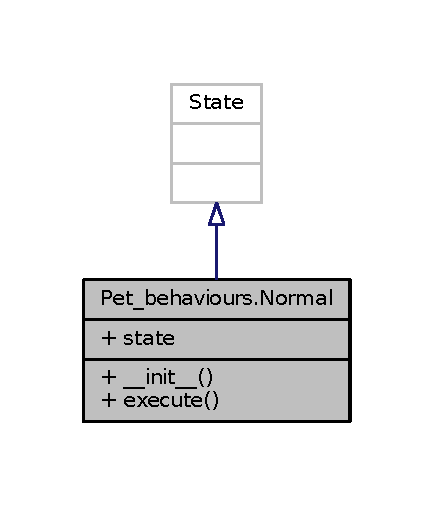
\includegraphics[width=208pt]{classPet__behaviours_1_1Normal__inherit__graph}
\end{center}
\end{figure}


Collaboration diagram for Pet\+\_\+behaviours.\+Normal\+:\nopagebreak
\begin{figure}[H]
\begin{center}
\leavevmode
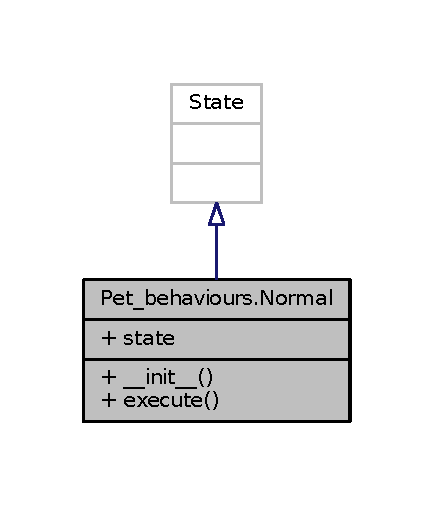
\includegraphics[width=208pt]{classPet__behaviours_1_1Normal__coll__graph}
\end{center}
\end{figure}
\subsection*{Public Member Functions}
\begin{DoxyCompactItemize}
\item 
def {\bfseries \+\_\+\+\_\+init\+\_\+\+\_\+} (self)\hypertarget{classPet__behaviours_1_1Normal_a04301ed05d5952e591268a758309862b}{}\label{classPet__behaviours_1_1Normal_a04301ed05d5952e591268a758309862b}

\item 
def {\bfseries execute} (self, userdata)\hypertarget{classPet__behaviours_1_1Normal_a2bbd4605a4cdc6dc02f5e80af5b614a0}{}\label{classPet__behaviours_1_1Normal_a2bbd4605a4cdc6dc02f5e80af5b614a0}

\end{DoxyCompactItemize}
\subsection*{Static Public Attributes}
\begin{DoxyCompactItemize}
\item 
\hyperlink{classPet__behaviours_1_1Normal_a8a500787fd6cc1891b861a4d11e8ca7f}{state} = rospy.\+get\+\_\+param(\textquotesingle{}state\textquotesingle{})
\begin{DoxyCompactList}\small\item\em check state \end{DoxyCompactList}\end{DoxyCompactItemize}


\subsection{Detailed Description}
\hyperlink{classPet__behaviours_1_1Normal}{Normal}\+: class that describes the \hyperlink{classPet__behaviours_1_1Normal}{Normal} state. 

Definition at line 112 of file Pet\+\_\+behaviours.\+py.



\subsection{Member Data Documentation}
\index{Pet\+\_\+behaviours\+::\+Normal@{Pet\+\_\+behaviours\+::\+Normal}!state@{state}}
\index{state@{state}!Pet\+\_\+behaviours\+::\+Normal@{Pet\+\_\+behaviours\+::\+Normal}}
\subsubsection[{\texorpdfstring{state}{state}}]{\setlength{\rightskip}{0pt plus 5cm}Pet\+\_\+behaviours.\+Normal.\+state = rospy.\+get\+\_\+param(\textquotesingle{}state\textquotesingle{})\hspace{0.3cm}{\ttfamily [static]}}\hypertarget{classPet__behaviours_1_1Normal_a8a500787fd6cc1891b861a4d11e8ca7f}{}\label{classPet__behaviours_1_1Normal_a8a500787fd6cc1891b861a4d11e8ca7f}


check state 

roam check the state 

Definition at line 124 of file Pet\+\_\+behaviours.\+py.



The documentation for this class was generated from the following file\+:\begin{DoxyCompactItemize}
\item 
scripts/\hyperlink{Pet__behaviours_8py}{Pet\+\_\+behaviours.\+py}\end{DoxyCompactItemize}

\hypertarget{classPet__behaviours_1_1Play}{}\section{Pet\+\_\+behaviours.\+Play Class Reference}
\label{classPet__behaviours_1_1Play}\index{Pet\+\_\+behaviours.\+Play@{Pet\+\_\+behaviours.\+Play}}


\hyperlink{classPet__behaviours_1_1Play}{Play}\+: class that describes the \hyperlink{classPet__behaviours_1_1Play}{Play} state.  




Inheritance diagram for Pet\+\_\+behaviours.\+Play\+:\nopagebreak
\begin{figure}[H]
\begin{center}
\leavevmode
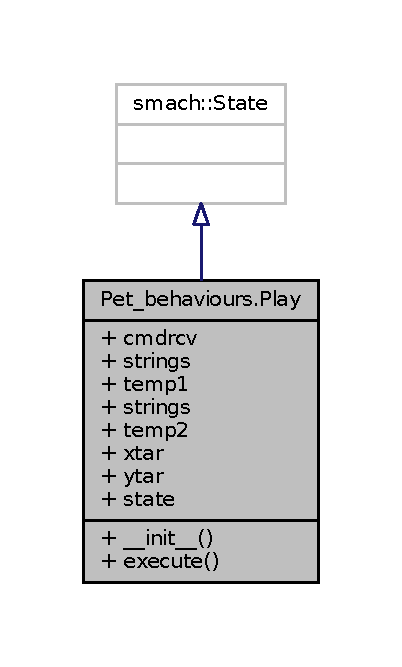
\includegraphics[width=193pt]{classPet__behaviours_1_1Play__inherit__graph}
\end{center}
\end{figure}


Collaboration diagram for Pet\+\_\+behaviours.\+Play\+:\nopagebreak
\begin{figure}[H]
\begin{center}
\leavevmode
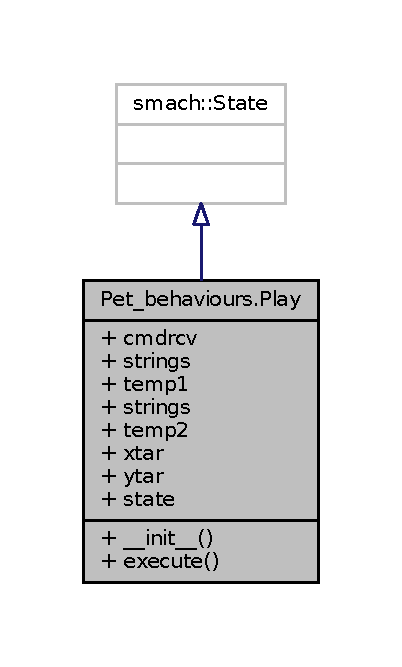
\includegraphics[width=193pt]{classPet__behaviours_1_1Play__coll__graph}
\end{center}
\end{figure}
\subsection*{Public Member Functions}
\begin{DoxyCompactItemize}
\item 
def {\bfseries \+\_\+\+\_\+init\+\_\+\+\_\+} (self)\hypertarget{classPet__behaviours_1_1Play_abaa16a6b254a58dfa47da4c3cca55b20}{}\label{classPet__behaviours_1_1Play_abaa16a6b254a58dfa47da4c3cca55b20}

\item 
def {\bfseries execute} (self, userdata)\hypertarget{classPet__behaviours_1_1Play_a03948eb0dd2c9595f88741a11199271a}{}\label{classPet__behaviours_1_1Play_a03948eb0dd2c9595f88741a11199271a}

\end{DoxyCompactItemize}
\subsection*{Static Public Attributes}
\begin{DoxyCompactItemize}
\item 
{\bfseries cmdrcv}\hypertarget{classPet__behaviours_1_1Play_aada475410ff2bedf7fd94f7aff1be5d9}{}\label{classPet__behaviours_1_1Play_aada475410ff2bedf7fd94f7aff1be5d9}

\item 
\hyperlink{classPet__behaviours_1_1Play_ad7ecb0f90069cd70ebc3f86f92b51415}{strings} = cmdrcv().status\hypertarget{classPet__behaviours_1_1Play_ad7ecb0f90069cd70ebc3f86f92b51415}{}\label{classPet__behaviours_1_1Play_ad7ecb0f90069cd70ebc3f86f92b51415}

\begin{DoxyCompactList}\small\item\em if the command is received Extract the command \end{DoxyCompactList}\item 
\hyperlink{classPet__behaviours_1_1Play_a0140f371bf2370c8f93925750383841f}{temp1} = strings.\+split(\char`\"{}$\vert$\char`\"{})
\begin{DoxyCompactList}\small\item\em Find if the command is empty. \end{DoxyCompactList}\item 
string {\bfseries strings} = \char`\"{}\char`\"{}\hypertarget{classPet__behaviours_1_1Play_a14f33bb8029ad809dce5dc5f3c52078f}{}\label{classPet__behaviours_1_1Play_a14f33bb8029ad809dce5dc5f3c52078f}

\item 
\hyperlink{classPet__behaviours_1_1Play_ae50b6080952ef514d49a0e56483ce25f}{temp2} = \hyperlink{classPet__behaviours_1_1Play_a0140f371bf2370c8f93925750383841f}{temp1}\mbox{[}i\mbox{]}.split(\char`\"{} \char`\"{})\hypertarget{classPet__behaviours_1_1Play_ae50b6080952ef514d49a0e56483ce25f}{}\label{classPet__behaviours_1_1Play_ae50b6080952ef514d49a0e56483ce25f}

\begin{DoxyCompactList}\small\item\em parse each command in x and y \end{DoxyCompactList}\item 
\hyperlink{classPet__behaviours_1_1Play_aa7e0891e996e7d38e850cc388516b0c7}{xtar} = int(\hyperlink{classPet__behaviours_1_1Play_ae50b6080952ef514d49a0e56483ce25f}{temp2}\mbox{[}0\mbox{]})
\begin{DoxyCompactList}\small\item\em go owner \end{DoxyCompactList}\item 
{\bfseries ytar} = int(\hyperlink{classPet__behaviours_1_1Play_ae50b6080952ef514d49a0e56483ce25f}{temp2}\mbox{[}1\mbox{]})\hypertarget{classPet__behaviours_1_1Play_ad298b18a3f0f68219a9d2abdfaf84e00}{}\label{classPet__behaviours_1_1Play_ad298b18a3f0f68219a9d2abdfaf84e00}

\item 
\hyperlink{classPet__behaviours_1_1Play_ad1cd8e207b954e328020bc5026bff92e}{state} = rospy.\+get\+\_\+param(\textquotesingle{}state\textquotesingle{})\hypertarget{classPet__behaviours_1_1Play_ad1cd8e207b954e328020bc5026bff92e}{}\label{classPet__behaviours_1_1Play_ad1cd8e207b954e328020bc5026bff92e}

\begin{DoxyCompactList}\small\item\em check the state \end{DoxyCompactList}\end{DoxyCompactItemize}


\subsection{Detailed Description}
\hyperlink{classPet__behaviours_1_1Play}{Play}\+: class that describes the \hyperlink{classPet__behaviours_1_1Play}{Play} state. 

Definition at line 131 of file Pet\+\_\+behaviours.\+py.



\subsection{Member Data Documentation}
\index{Pet\+\_\+behaviours\+::\+Play@{Pet\+\_\+behaviours\+::\+Play}!temp1@{temp1}}
\index{temp1@{temp1}!Pet\+\_\+behaviours\+::\+Play@{Pet\+\_\+behaviours\+::\+Play}}
\subsubsection[{\texorpdfstring{temp1}{temp1}}]{\setlength{\rightskip}{0pt plus 5cm}Pet\+\_\+behaviours.\+Play.\+temp1 = strings.\+split(\char`\"{}$\vert$\char`\"{})\hspace{0.3cm}{\ttfamily [static]}}\hypertarget{classPet__behaviours_1_1Play_a0140f371bf2370c8f93925750383841f}{}\label{classPet__behaviours_1_1Play_a0140f371bf2370c8f93925750383841f}


Find if the command is empty. 

if command received 

Definition at line 147 of file Pet\+\_\+behaviours.\+py.

\index{Pet\+\_\+behaviours\+::\+Play@{Pet\+\_\+behaviours\+::\+Play}!xtar@{xtar}}
\index{xtar@{xtar}!Pet\+\_\+behaviours\+::\+Play@{Pet\+\_\+behaviours\+::\+Play}}
\subsubsection[{\texorpdfstring{xtar}{xtar}}]{\setlength{\rightskip}{0pt plus 5cm}Pet\+\_\+behaviours.\+Play.\+xtar = int({\bf temp2}\mbox{[}0\mbox{]})\hspace{0.3cm}{\ttfamily [static]}}\hypertarget{classPet__behaviours_1_1Play_aa7e0891e996e7d38e850cc388516b0c7}{}\label{classPet__behaviours_1_1Play_aa7e0891e996e7d38e850cc388516b0c7}


go owner 

Check if in normal or not.

Return to the owner when all commands are executed 

Definition at line 153 of file Pet\+\_\+behaviours.\+py.



The documentation for this class was generated from the following file\+:\begin{DoxyCompactItemize}
\item 
scripts/\hyperlink{Pet__behaviours_8py}{Pet\+\_\+behaviours.\+py}\end{DoxyCompactItemize}

\hypertarget{classPet__behaviours_1_1Sleep}{}\section{Pet\+\_\+behaviours.\+Sleep Class Reference}
\label{classPet__behaviours_1_1Sleep}\index{Pet\+\_\+behaviours.\+Sleep@{Pet\+\_\+behaviours.\+Sleep}}


\hyperlink{classPet__behaviours_1_1Sleep}{Sleep}\+: class that describes the \hyperlink{classPet__behaviours_1_1Sleep}{Sleep} state.  




Inheritance diagram for Pet\+\_\+behaviours.\+Sleep\+:\nopagebreak
\begin{figure}[H]
\begin{center}
\leavevmode
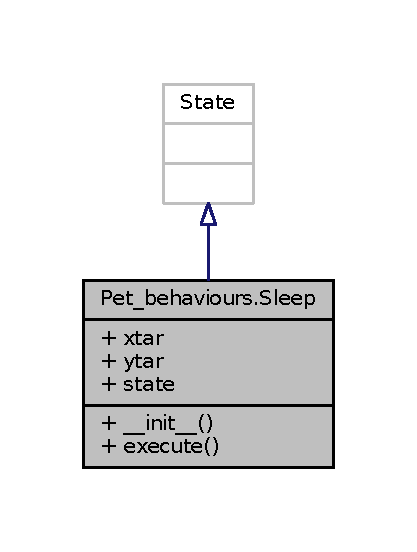
\includegraphics[width=200pt]{classPet__behaviours_1_1Sleep__inherit__graph}
\end{center}
\end{figure}


Collaboration diagram for Pet\+\_\+behaviours.\+Sleep\+:\nopagebreak
\begin{figure}[H]
\begin{center}
\leavevmode
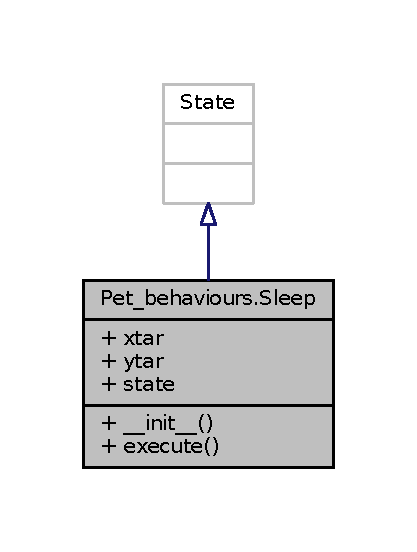
\includegraphics[width=200pt]{classPet__behaviours_1_1Sleep__coll__graph}
\end{center}
\end{figure}
\subsection*{Public Member Functions}
\begin{DoxyCompactItemize}
\item 
def {\bfseries \+\_\+\+\_\+init\+\_\+\+\_\+} (self)\hypertarget{classPet__behaviours_1_1Sleep_a4c496191e2c51bf2984208d180e1fd99}{}\label{classPet__behaviours_1_1Sleep_a4c496191e2c51bf2984208d180e1fd99}

\item 
def {\bfseries execute} (self, userdata)\hypertarget{classPet__behaviours_1_1Sleep_a952790c46209d96b95cb0c63de329b97}{}\label{classPet__behaviours_1_1Sleep_a952790c46209d96b95cb0c63de329b97}

\end{DoxyCompactItemize}
\subsection*{Static Public Attributes}
\begin{DoxyCompactItemize}
\item 
\hyperlink{classPet__behaviours_1_1Sleep_a643e30c580a0274a40c28847a1c9e445}{xtar} = rospy.\+get\+\_\+param(\textquotesingle{}home/x\textquotesingle{})\hypertarget{classPet__behaviours_1_1Sleep_a643e30c580a0274a40c28847a1c9e445}{}\label{classPet__behaviours_1_1Sleep_a643e30c580a0274a40c28847a1c9e445}

\begin{DoxyCompactList}\small\item\em while not at home \end{DoxyCompactList}\item 
{\bfseries ytar} = rospy.\+get\+\_\+param(\textquotesingle{}home/y\textquotesingle{})\hypertarget{classPet__behaviours_1_1Sleep_acff6bf9f7c507069469110129bce78fd}{}\label{classPet__behaviours_1_1Sleep_acff6bf9f7c507069469110129bce78fd}

\item 
\hyperlink{classPet__behaviours_1_1Sleep_a896626409cc2d477e99165f69de520de}{state} = rospy.\+get\+\_\+param(\textquotesingle{}state\textquotesingle{})
\begin{DoxyCompactList}\small\item\em if sleep state activated \end{DoxyCompactList}\end{DoxyCompactItemize}


\subsection{Detailed Description}
\hyperlink{classPet__behaviours_1_1Sleep}{Sleep}\+: class that describes the \hyperlink{classPet__behaviours_1_1Sleep}{Sleep} state. 

Definition at line 88 of file Pet\+\_\+behaviours.\+py.



\subsection{Member Data Documentation}
\index{Pet\+\_\+behaviours\+::\+Sleep@{Pet\+\_\+behaviours\+::\+Sleep}!state@{state}}
\index{state@{state}!Pet\+\_\+behaviours\+::\+Sleep@{Pet\+\_\+behaviours\+::\+Sleep}}
\subsubsection[{\texorpdfstring{state}{state}}]{\setlength{\rightskip}{0pt plus 5cm}Pet\+\_\+behaviours.\+Sleep.\+state = rospy.\+get\+\_\+param(\textquotesingle{}state\textquotesingle{})\hspace{0.3cm}{\ttfamily [static]}}\hypertarget{classPet__behaviours_1_1Sleep_a896626409cc2d477e99165f69de520de}{}\label{classPet__behaviours_1_1Sleep_a896626409cc2d477e99165f69de520de}


if sleep state activated 

change state if not sleep 

Definition at line 103 of file Pet\+\_\+behaviours.\+py.



The documentation for this class was generated from the following file\+:\begin{DoxyCompactItemize}
\item 
scripts/\hyperlink{Pet__behaviours_8py}{Pet\+\_\+behaviours.\+py}\end{DoxyCompactItemize}

\chapter{File Documentation}
\hypertarget{Command__giver_8py}{}\section{scripts/\+Command\+\_\+giver.py File Reference}
\label{Command__giver_8py}\index{scripts/\+Command\+\_\+giver.\+py@{scripts/\+Command\+\_\+giver.\+py}}


Component that gives command either randomly generated or given by a user, switching between the two.  


\subsection*{Variables}
\begin{DoxyCompactItemize}
\item 
\hyperlink{Command__giver_8py_a4a6d5cbbee4af6d7048bd06047255889}{Command\+\_\+giver.\+pub} = rospy.\+Publisher(\char`\"{}commander\char`\"{},String,queue\+\_\+size=10)
\begin{DoxyCompactList}\small\item\em Variable declaration. \end{DoxyCompactList}\item 
int {\bfseries Command\+\_\+giver.\+cmd\+\_\+gen} = 0\hypertarget{Command__giver_8py_a803b2b7ff72cc1b18c419be9a062021e}{}\label{Command__giver_8py_a803b2b7ff72cc1b18c419be9a062021e}

\item 
\hyperlink{Command__giver_8py_a3fc07d631a374497e2a0fccc8bb1ccdd}{Command\+\_\+giver.\+value} = random.\+randrange(30,45,5)
\begin{DoxyCompactList}\small\item\em Concatenate a lis t of commands. \end{DoxyCompactList}\item 
string {\bfseries Command\+\_\+giver.\+strings} = \char`\"{}\char`\"{}\hypertarget{Command__giver_8py_a7978b9d5f6b82ba4ee7dc49d2453e970}{}\label{Command__giver_8py_a7978b9d5f6b82ba4ee7dc49d2453e970}

\item 
{\bfseries Command\+\_\+giver.\+leng} = random.\+randrange(1,5,1)\hypertarget{Command__giver_8py_a025a1b6259531fe33224caac39ef4b7b}{}\label{Command__giver_8py_a025a1b6259531fe33224caac39ef4b7b}

\item 
\hyperlink{Command__giver_8py_ab183e03b2130f54244266f032764fcd0}{Command\+\_\+giver.\+xtar} = random.\+randrange(1,11,1)\hypertarget{Command__giver_8py_ab183e03b2130f54244266f032764fcd0}{}\label{Command__giver_8py_ab183e03b2130f54244266f032764fcd0}

\begin{DoxyCompactList}\small\item\em choose a target inside the map \end{DoxyCompactList}\item 
{\bfseries Command\+\_\+giver.\+ytar} = random.\+randrange(1,11,1)\hypertarget{Command__giver_8py_a1a218322646e0f384ca7874f04e60a48}{}\label{Command__giver_8py_a1a218322646e0f384ca7874f04e60a48}

\end{DoxyCompactItemize}


\subsection{Detailed Description}
Component that gives command either randomly generated or given by a user, switching between the two. 

Details\+: This component is the one that inputs commands inside the pet\+\_\+simulation, either it randomly generates random string command or receives them from the user 

\subsection{Variable Documentation}
\index{Command\+\_\+giver.\+py@{Command\+\_\+giver.\+py}!pub@{pub}}
\index{pub@{pub}!Command\+\_\+giver.\+py@{Command\+\_\+giver.\+py}}
\subsubsection[{\texorpdfstring{pub}{pub}}]{\setlength{\rightskip}{0pt plus 5cm}Command\+\_\+giver.\+pub = rospy.\+Publisher(\char`\"{}commander\char`\"{},String,queue\+\_\+size=10)}\hypertarget{Command__giver_8py_file_a4a6d5cbbee4af6d7048bd06047255889}{}\label{Command__giver_8py_file_a4a6d5cbbee4af6d7048bd06047255889}


Variable declaration. 

Main function declaration Init the ros node 

Definition at line 25 of file Command\+\_\+giver.\+py.

\index{Command\+\_\+giver.\+py@{Command\+\_\+giver.\+py}!value@{value}}
\index{value@{value}!Command\+\_\+giver.\+py@{Command\+\_\+giver.\+py}}
\subsubsection[{\texorpdfstring{value}{value}}]{\setlength{\rightskip}{0pt plus 5cm}Command\+\_\+giver.\+value = random.\+randrange(30,45,5)}\hypertarget{Command__giver_8py_file_a3fc07d631a374497e2a0fccc8bb1ccdd}{}\label{Command__giver_8py_file_a3fc07d631a374497e2a0fccc8bb1ccdd}


Concatenate a lis t of commands. 

chose whether to point or tell to go 

Definition at line 29 of file Command\+\_\+giver.\+py.


\hypertarget{Pet__behaviours_8py}{}\section{scripts/\+Pet\+\_\+behaviours.py File Reference}
\label{Pet__behaviours_8py}\index{scripts/\+Pet\+\_\+behaviours.\+py@{scripts/\+Pet\+\_\+behaviours.\+py}}


Pet state machine.  


\subsection*{Classes}
\begin{DoxyCompactItemize}
\item 
class \hyperlink{classPet__behaviours_1_1Sleep}{Pet\+\_\+behaviours.\+Sleep}
\begin{DoxyCompactList}\small\item\em \hyperlink{classPet__behaviours_1_1Sleep}{Sleep}\+: class that describes the \hyperlink{classPet__behaviours_1_1Sleep}{Sleep} state. \end{DoxyCompactList}\item 
class \hyperlink{classPet__behaviours_1_1Normal}{Pet\+\_\+behaviours.\+Normal}
\begin{DoxyCompactList}\small\item\em \hyperlink{classPet__behaviours_1_1Normal}{Normal}\+: class that describes the \hyperlink{classPet__behaviours_1_1Normal}{Normal} state. \end{DoxyCompactList}\item 
class \hyperlink{classPet__behaviours_1_1Play}{Pet\+\_\+behaviours.\+Play}
\begin{DoxyCompactList}\small\item\em \hyperlink{classPet__behaviours_1_1Play}{Play}\+: class that describes the \hyperlink{classPet__behaviours_1_1Play}{Play} state. \end{DoxyCompactList}\end{DoxyCompactItemize}
\subsection*{Functions}
\begin{DoxyCompactItemize}
\item 
def \hyperlink{Pet__behaviours_8py_ac416f11d9f795118d4795f22f4b43234}{Pet\+\_\+behaviours.\+go\+\_\+to\+\_\+target} (xtar, ytar)\hypertarget{Pet__behaviours_8py_ac416f11d9f795118d4795f22f4b43234}{}\label{Pet__behaviours_8py_ac416f11d9f795118d4795f22f4b43234}

\begin{DoxyCompactList}\small\item\em go\+\_\+to\+\_\+target\+: function to go to a target specified by the coordinates (xtar,ytar) \end{DoxyCompactList}\item 
def \hyperlink{Pet__behaviours_8py_aa13193e5cc4138c5687609d1f644cc27}{Pet\+\_\+behaviours.\+roam} ()\hypertarget{Pet__behaviours_8py_aa13193e5cc4138c5687609d1f644cc27}{}\label{Pet__behaviours_8py_aa13193e5cc4138c5687609d1f644cc27}

\begin{DoxyCompactList}\small\item\em roam\+: function to simulate the roaming behaviour of normal \end{DoxyCompactList}\item 
def \hyperlink{Pet__behaviours_8py_a34ab7be91b1041bbd6b691f9a0a72b9c}{Pet\+\_\+behaviours.\+simcallback} (data)\hypertarget{Pet__behaviours_8py_a34ab7be91b1041bbd6b691f9a0a72b9c}{}\label{Pet__behaviours_8py_a34ab7be91b1041bbd6b691f9a0a72b9c}

\begin{DoxyCompactList}\small\item\em simcallback\+: callback for the simulated pet position \end{DoxyCompactList}\end{DoxyCompactItemize}
\subsection*{Variables}
\begin{DoxyCompactItemize}
\item 
int \hyperlink{Pet__behaviours_8py_aa2ca9b121e3facefb6575cedc3612b4b}{Pet\+\_\+behaviours.\+x} = 0\hypertarget{Pet__behaviours_8py_aa2ca9b121e3facefb6575cedc3612b4b}{}\label{Pet__behaviours_8py_aa2ca9b121e3facefb6575cedc3612b4b}

\begin{DoxyCompactList}\small\item\em Variable definition global x position. \end{DoxyCompactList}\item 
int \hyperlink{Pet__behaviours_8py_afb7e96c8fdcc67add7d701aca7ba5573}{Pet\+\_\+behaviours.\+y} = 0\hypertarget{Pet__behaviours_8py_afb7e96c8fdcc67add7d701aca7ba5573}{}\label{Pet__behaviours_8py_afb7e96c8fdcc67add7d701aca7ba5573}

\begin{DoxyCompactList}\small\item\em global y position \end{DoxyCompactList}\item 
int \hyperlink{Pet__behaviours_8py_aee2de25e04c0eb0fd3fc0dc3260a6f46}{Pet\+\_\+behaviours.\+theta} = 0\hypertarget{Pet__behaviours_8py_aee2de25e04c0eb0fd3fc0dc3260a6f46}{}\label{Pet__behaviours_8py_aee2de25e04c0eb0fd3fc0dc3260a6f46}

\begin{DoxyCompactList}\small\item\em global theta position \end{DoxyCompactList}\item 
int \hyperlink{Pet__behaviours_8py_aa0d0b7436444bfcec6f8cf6a24f051ca}{Pet\+\_\+behaviours.\+comm} = 0\hypertarget{Pet__behaviours_8py_aa0d0b7436444bfcec6f8cf6a24f051ca}{}\label{Pet__behaviours_8py_aa0d0b7436444bfcec6f8cf6a24f051ca}

\begin{DoxyCompactList}\small\item\em command received \end{DoxyCompactList}\item 
int \hyperlink{Pet__behaviours_8py_ae0261eeb91fe5de1751fe9cc1935c8f4}{Pet\+\_\+behaviours.\+xt} = 0\hypertarget{Pet__behaviours_8py_ae0261eeb91fe5de1751fe9cc1935c8f4}{}\label{Pet__behaviours_8py_ae0261eeb91fe5de1751fe9cc1935c8f4}

\begin{DoxyCompactList}\small\item\em x target \end{DoxyCompactList}\item 
int \hyperlink{Pet__behaviours_8py_a168a8f64fdcb791cb4ae88efb5232fc8}{Pet\+\_\+behaviours.\+yt} = 0\hypertarget{Pet__behaviours_8py_a168a8f64fdcb791cb4ae88efb5232fc8}{}\label{Pet__behaviours_8py_a168a8f64fdcb791cb4ae88efb5232fc8}

\begin{DoxyCompactList}\small\item\em y target \end{DoxyCompactList}\item 
float \hyperlink{Pet__behaviours_8py_a05cba7438bef49d22f2c83249f468514}{Pet\+\_\+behaviours.\+timer} = 0.\+5\hypertarget{Pet__behaviours_8py_a05cba7438bef49d22f2c83249f468514}{}\label{Pet__behaviours_8py_a05cba7438bef49d22f2c83249f468514}

\begin{DoxyCompactList}\small\item\em delay timer \end{DoxyCompactList}\item 
\hyperlink{Pet__behaviours_8py_a88c2949521b61c538c120dd9c08bf4da}{Pet\+\_\+behaviours.\+colorserv} = rospy.\+Service\+Proxy(\textquotesingle{}/turtle1/set\+\_\+pen\textquotesingle{}, Set\+Pen)
\begin{DoxyCompactList}\small\item\em Main function declaration. \end{DoxyCompactList}\item 
{\bfseries Pet\+\_\+behaviours.\+teleportabs} = rospy.\+Service\+Proxy(\textquotesingle{}/turtle1/teleport\+\_\+absolute\textquotesingle{}, Teleport\+Absolute)\hypertarget{Pet__behaviours_8py_a06621618a7dee5915598d47a610431e4}{}\label{Pet__behaviours_8py_a06621618a7dee5915598d47a610431e4}

\item 
{\bfseries Pet\+\_\+behaviours.\+resets} = rospy.\+Service\+Proxy(\textquotesingle{}/clear\textquotesingle{},Empty)\hypertarget{Pet__behaviours_8py_acb6617ff10cb1900363cbec0b0198c06}{}\label{Pet__behaviours_8py_acb6617ff10cb1900363cbec0b0198c06}

\item 
\hyperlink{Pet__behaviours_8py_afeb58c147d02f423a6007b511c89cf51}{Pet\+\_\+behaviours.\+sm\+\_\+s\+\_\+a} = smach.\+State\+Machine(outcomes=\mbox{[}\textquotesingle{}outcome4\textquotesingle{}\mbox{]})\hypertarget{Pet__behaviours_8py_afeb58c147d02f423a6007b511c89cf51}{}\label{Pet__behaviours_8py_afeb58c147d02f423a6007b511c89cf51}

\begin{DoxyCompactList}\small\item\em Create a S\+M\+A\+CH state machine. \end{DoxyCompactList}\item 
\hyperlink{Pet__behaviours_8py_a30f56769923a0b61fc3be32e119a2afa}{Pet\+\_\+behaviours.\+transitions}
\begin{DoxyCompactList}\small\item\em Open the container. \end{DoxyCompactList}\item 
\hyperlink{Pet__behaviours_8py_af096456cf166ae9c4c159843b5ea1421}{Pet\+\_\+behaviours.\+outcome} = sm\+\_\+s\+\_\+a.\+execute()\hypertarget{Pet__behaviours_8py_af096456cf166ae9c4c159843b5ea1421}{}\label{Pet__behaviours_8py_af096456cf166ae9c4c159843b5ea1421}

\begin{DoxyCompactList}\small\item\em Execute S\+M\+A\+CH plan. \end{DoxyCompactList}\end{DoxyCompactItemize}


\subsection{Detailed Description}
Pet state machine. 

Details\+: This component simulate the behaviour state machine 

\subsection{Variable Documentation}
\index{Pet\+\_\+behaviours.\+py@{Pet\+\_\+behaviours.\+py}!colorserv@{colorserv}}
\index{colorserv@{colorserv}!Pet\+\_\+behaviours.\+py@{Pet\+\_\+behaviours.\+py}}
\subsubsection[{\texorpdfstring{colorserv}{colorserv}}]{\setlength{\rightskip}{0pt plus 5cm}Pet\+\_\+behaviours.\+colorserv = rospy.\+Service\+Proxy(\textquotesingle{}/turtle1/set\+\_\+pen\textquotesingle{}, Set\+Pen)}\hypertarget{Pet__behaviours_8py_file_a88c2949521b61c538c120dd9c08bf4da}{}\label{Pet__behaviours_8py_file_a88c2949521b61c538c120dd9c08bf4da}


Main function declaration. 

Init the ros node 

Definition at line 210 of file Pet\+\_\+behaviours.\+py.

\index{Pet\+\_\+behaviours.\+py@{Pet\+\_\+behaviours.\+py}!transitions@{transitions}}
\index{transitions@{transitions}!Pet\+\_\+behaviours.\+py@{Pet\+\_\+behaviours.\+py}}
\subsubsection[{\texorpdfstring{transitions}{transitions}}]{\setlength{\rightskip}{0pt plus 5cm}Pet\+\_\+behaviours.\+transitions}\hypertarget{Pet__behaviours_8py_file_a30f56769923a0b61fc3be32e119a2afa}{}\label{Pet__behaviours_8py_file_a30f56769923a0b61fc3be32e119a2afa}


Open the container. 

Add states to the container.

Add states to the container 

Definition at line 226 of file Pet\+\_\+behaviours.\+py.


\hypertarget{Pet__logic_8py}{}\section{scripts/\+Pet\+\_\+logic.py File Reference}
\label{Pet__logic_8py}\index{scripts/\+Pet\+\_\+logic.\+py@{scripts/\+Pet\+\_\+logic.\+py}}


Pet logic.  


\subsection*{Functions}
\begin{DoxyCompactItemize}
\item 
def \hyperlink{Pet__logic_8py_a87af419094566f200ba47226d9064173}{Pet\+\_\+logic.\+srv\+Callback} (req)\hypertarget{Pet__logic_8py_a87af419094566f200ba47226d9064173}{}\label{Pet__logic_8py_a87af419094566f200ba47226d9064173}

\begin{DoxyCompactList}\small\item\em srv\+Callback\+: service function to send the command to Pet\+\_\+behaviours \end{DoxyCompactList}\item 
def \hyperlink{Pet__logic_8py_a0df6eab5500aa07da057103543f7c926}{Pet\+\_\+logic.\+com\+Callback} (msg)\hypertarget{Pet__logic_8py_a0df6eab5500aa07da057103543f7c926}{}\label{Pet__logic_8py_a0df6eab5500aa07da057103543f7c926}

\begin{DoxyCompactList}\small\item\em com\+Callback\+: The callback that receive the command from the commander and convert them to a compliant format \end{DoxyCompactList}\end{DoxyCompactItemize}
\subsection*{Variables}
\begin{DoxyCompactItemize}
\item 
list \hyperlink{Pet__logic_8py_a5b70925b74d5b83fc97a0775323124da}{Pet\+\_\+logic.\+command} = \mbox{[}$\,$\mbox{]}\hypertarget{Pet__logic_8py_a5b70925b74d5b83fc97a0775323124da}{}\label{Pet__logic_8py_a5b70925b74d5b83fc97a0775323124da}

\begin{DoxyCompactList}\small\item\em Variable declaration Command string. \end{DoxyCompactList}\item 
int \hyperlink{Pet__logic_8py_ab572ac6b85eef0a9c39b12ae349a3ca2}{Pet\+\_\+logic.\+msg\+\_\+received} = 1\hypertarget{Pet__logic_8py_ab572ac6b85eef0a9c39b12ae349a3ca2}{}\label{Pet__logic_8py_ab572ac6b85eef0a9c39b12ae349a3ca2}

\begin{DoxyCompactList}\small\item\em variable if a message is received \end{DoxyCompactList}\item 
\hyperlink{Pet__logic_8py_a9e187db9dfc2442b9b753be0df7b8c49}{Pet\+\_\+logic.\+s} = rospy.\+Service(\textquotesingle{}commandsrv\textquotesingle{}, Get\+Status, srv\+Callback)
\begin{DoxyCompactList}\small\item\em Main function declaration. \end{DoxyCompactList}\item 
{\bfseries Pet\+\_\+logic.\+rate} = rospy.\+Rate(5)\hypertarget{Pet__logic_8py_ab143a04efb8b92bed19f2526dd9d8772}{}\label{Pet__logic_8py_ab143a04efb8b92bed19f2526dd9d8772}

\item 
{\bfseries Pet\+\_\+logic.\+value} = random.\+randrange(15,45,5)\hypertarget{Pet__logic_8py_aed4ef665aac366519b41d46be4541559}{}\label{Pet__logic_8py_aed4ef665aac366519b41d46be4541559}

\item 
{\bfseries Pet\+\_\+logic.\+state} = rospy.\+get\+\_\+param(\textquotesingle{}state\textquotesingle{})\hypertarget{Pet__logic_8py_aa4e891065db5c8c8aa1f89ef4cc3da24}{}\label{Pet__logic_8py_aa4e891065db5c8c8aa1f89ef4cc3da24}

\end{DoxyCompactItemize}


\subsection{Detailed Description}
Pet logic. 

Details\+: This component is the one that receives command, convert the command in a more compliant format and change state 

\subsection{Variable Documentation}
\index{Pet\+\_\+logic.\+py@{Pet\+\_\+logic.\+py}!s@{s}}
\index{s@{s}!Pet\+\_\+logic.\+py@{Pet\+\_\+logic.\+py}}
\subsubsection[{\texorpdfstring{s}{s}}]{\setlength{\rightskip}{0pt plus 5cm}Pet\+\_\+logic.\+s = rospy.\+Service(\textquotesingle{}commandsrv\textquotesingle{}, Get\+Status, srv\+Callback)}\hypertarget{Pet__logic_8py_file_a9e187db9dfc2442b9b753be0df7b8c49}{}\label{Pet__logic_8py_file_a9e187db9dfc2442b9b753be0df7b8c49}


Main function declaration. 

Init the ros nodek 

Definition at line 83 of file Pet\+\_\+logic.\+py.


\hypertarget{state__outfit__simulator__node_8py}{}\section{scripts/state\+\_\+outfit\+\_\+simulator\+\_\+node.py File Reference}
\label{state__outfit__simulator__node_8py}\index{scripts/state\+\_\+outfit\+\_\+simulator\+\_\+node.\+py@{scripts/state\+\_\+outfit\+\_\+simulator\+\_\+node.\+py}}


Test component of the pet state machine output to the turtlesim environment.  


\subsection*{Functions}
\begin{DoxyCompactItemize}
\item 
def \hyperlink{state__outfit__simulator__node_8py_a526b0547c2baea1fd179bac43de0e7ae}{state\+\_\+outfit\+\_\+simulator\+\_\+node.\+simcallback} (data)\hypertarget{state__outfit__simulator__node_8py_a526b0547c2baea1fd179bac43de0e7ae}{}\label{state__outfit__simulator__node_8py_a526b0547c2baea1fd179bac43de0e7ae}

\begin{DoxyCompactList}\small\item\em simcallback\+: pose response from turtlesim \end{DoxyCompactList}\end{DoxyCompactItemize}
\subsection*{Variables}
\begin{DoxyCompactItemize}
\item 
int \hyperlink{state__outfit__simulator__node_8py_aacff9df64f9423202e945a99ee675e51}{state\+\_\+outfit\+\_\+simulator\+\_\+node.\+x} = 0\hypertarget{state__outfit__simulator__node_8py_aacff9df64f9423202e945a99ee675e51}{}\label{state__outfit__simulator__node_8py_aacff9df64f9423202e945a99ee675e51}

\begin{DoxyCompactList}\small\item\em global x position \end{DoxyCompactList}\item 
int \hyperlink{state__outfit__simulator__node_8py_a7b0904aaae9f6d6c72e9ae95d0ab7cbb}{state\+\_\+outfit\+\_\+simulator\+\_\+node.\+y} = 0\hypertarget{state__outfit__simulator__node_8py_a7b0904aaae9f6d6c72e9ae95d0ab7cbb}{}\label{state__outfit__simulator__node_8py_a7b0904aaae9f6d6c72e9ae95d0ab7cbb}

\begin{DoxyCompactList}\small\item\em global y position \end{DoxyCompactList}\item 
\hyperlink{state__outfit__simulator__node_8py_a84d2bdc16f93ea81aa23e3be7ae1ad09}{state\+\_\+outfit\+\_\+simulator\+\_\+node.\+teleportabs} = rospy.\+Service\+Proxy(\textquotesingle{}/turtle1/teleport\+\_\+absolute\textquotesingle{}, Teleport\+Absolute)
\begin{DoxyCompactList}\small\item\em Main function declaration. \end{DoxyCompactList}\item 
{\bfseries state\+\_\+outfit\+\_\+simulator\+\_\+node.\+resets} = rospy.\+Service\+Proxy(\textquotesingle{}/clear\textquotesingle{},Empty)\hypertarget{state__outfit__simulator__node_8py_aa318caca530c214094bef4f8b2b714b7}{}\label{state__outfit__simulator__node_8py_aa318caca530c214094bef4f8b2b714b7}

\item 
{\bfseries state\+\_\+outfit\+\_\+simulator\+\_\+node.\+rate} = rospy.\+Rate(5)\hypertarget{state__outfit__simulator__node_8py_a193f4f89f10eb0b85c13ca2cf66d6003}{}\label{state__outfit__simulator__node_8py_a193f4f89f10eb0b85c13ca2cf66d6003}

\item 
{\bfseries state\+\_\+outfit\+\_\+simulator\+\_\+node.\+dx} = random.\+randint(-\/1,1)\hypertarget{state__outfit__simulator__node_8py_ad751a0e2d601aa51e0f8dcc3c0cf2463}{}\label{state__outfit__simulator__node_8py_ad751a0e2d601aa51e0f8dcc3c0cf2463}

\item 
{\bfseries state\+\_\+outfit\+\_\+simulator\+\_\+node.\+dy} = random.\+randint(-\/1,1)\hypertarget{state__outfit__simulator__node_8py_a50e0ce3202b7e8226b193095f7b173b3}{}\label{state__outfit__simulator__node_8py_a50e0ce3202b7e8226b193095f7b173b3}

\end{DoxyCompactItemize}


\subsection{Detailed Description}
Test component of the pet state machine output to the turtlesim environment. 

Details\+: This component simulate the command from the pet state machine and relays them to the turtlesim environment reading the current position of the turtlesim pet 

\subsection{Variable Documentation}
\index{state\+\_\+outfit\+\_\+simulator\+\_\+node.\+py@{state\+\_\+outfit\+\_\+simulator\+\_\+node.\+py}!teleportabs@{teleportabs}}
\index{teleportabs@{teleportabs}!state\+\_\+outfit\+\_\+simulator\+\_\+node.\+py@{state\+\_\+outfit\+\_\+simulator\+\_\+node.\+py}}
\subsubsection[{\texorpdfstring{teleportabs}{teleportabs}}]{\setlength{\rightskip}{0pt plus 5cm}state\+\_\+outfit\+\_\+simulator\+\_\+node.\+teleportabs = rospy.\+Service\+Proxy(\textquotesingle{}/turtle1/teleport\+\_\+absolute\textquotesingle{}, Teleport\+Absolute)}\hypertarget{state__outfit__simulator__node_8py_file_a84d2bdc16f93ea81aa23e3be7ae1ad09}{}\label{state__outfit__simulator__node_8py_file_a84d2bdc16f93ea81aa23e3be7ae1ad09}


Main function declaration. 

Init the ros node teleportation function 

Definition at line 47 of file state\+\_\+outfit\+\_\+simulator\+\_\+node.\+py.


%--- End generated contents ---

% Index
\backmatter
\newpage
\phantomsection
\clearemptydoublepage
\addcontentsline{toc}{chapter}{Index}
\printindex

\end{document}
